\documentclass[fleqn]{MJD}

\usepackage{cancel}
\usepackage{cleveref}
\usepackage{titlesec}
\usepackage{hyperref}
%\colorsections
%\bluelinks
\newcommand{\problem}[1]{\chapter{Problem #1}}
\newcommand{\subproblem}[2]{\section{(#1)~ #2}}
\newcommand{\subsubproblem}[2]{\subsection{ #1)~ #2}}
\newcommand{\U}{\cup}
\renewcommand{\S}{\mathcal{S}}
\renewcommand{\s}{\subset}
\renewcommand{\equiv}{\Leftrightarrow}
\newcommand{\0}{\emptyset}
\newcommand{\imp}{\Rightarrow}
\newcommand{\Usum}{\bigcup\limits_{i=1}^\infty}
\newcommand{\intsum}{\bigcup\limits_{i=1}^\infty}
\newcommand{\infsum}{\sum\limits_{i=1}^\infty}
\newcommand{\sets}{\{A_1, A_2 \dots\} }
\newcommand{\nsets}{\{A_1, \dots, A_n \} }

\titleformat{\chapter}[display]
  {\normalfont\bfseries}{}{0pt}{\LARGE}
  
\graphicspath{ {../} }

%%%%%%%%%%%%%%%%%%%%%%%%%%%%%%%%%%%%
\begin{document}
\lstset{language=Python}
\titleAT[CS 224N: Assignment 2]{Peter888@stanford.edu}
%-------------------------------------
\problem{1: Tensorflow Softmax (25 points)}
%-------------------------------------

%----------------------
\subproblem{a}{Implement Softmax use Tensorflow (5 points, coding)}
\noindent\textbf{Answer:} \\
\noindent See code: $\sim$\verb|/q1_softmax.py|.

\vskip5em

%----------------------
\subproblem{b}{Implement Cross-Entropy use Tensorflow (5 points, coding)}
\noindent \textbf{Answer:} \\

\noindent See code: $\sim$\verb|/q1_softmax.py|.

\vskip5em
%----------------------
\subproblem{c}{Tensorflow Placeholder and Feed Dictionary (5 points, coding/written)}
\noindent \textbf{Answer:} \\

\noindent See code: $\sim$\verb|/q1_classifier.py|. 
\vskip3em
\textit {Explanation:}

\vskip5em
\newpage

%----------------------
\subproblem{d}{Implement Classifier (5 points, coding)}
\noindent\textbf{Answer:} \\
\noindent See code: $\sim$\verb|/q1_classifier.py|.

\vskip5em
%----------------------
\subproblem{e}{Implement Model (5 points, coding/written)}
\noindent\textbf{Answer:} \\
\noindent See code: $\sim$\verb|/q1_classifier.py|. 
\vskip3em
\textit {Explanation:}

\vskip5em
%-------------------------------------
\problem{2: Neural Transition-Based Dependency Parsing (50 points + 2 bonus points)}
%-------------------------------------

%----------------------
\subproblem{a}{Dependency Parsing (6 points, written)}

\noindent \textbf{Answer:}


\begin{table}[!htbp]
	\centering
	\small
\begin{tabular}{l|l|l|l}
\textbf{stack} 						& \textbf{buffer}							& \textbf{ new dependency}	& \textbf{transition} 	\\ \hline 
$[ROOT]$ 							& $[I, parsed, this, sentence, correctly]$  &  							& Initial Configuration \\ 
$[ROOT, I]$ 						& $[parsed, this, sentence, correctly]$ 	&  							& \verb|SHIFT|  		\\ 
$[ROOT, I, parsed]$ 				& $[this, sentence, correctly]$ 			&  							& \verb|SHIFT|  		\\ 
$[ROOT, parsed]$ 					& $[this, sentence, correctly]$ 			& parsed $\rightarrow$ I 	& \verb|LEFT-ARC| 		\\ \hline
$[ROOT, parsed, this]$				& $[sentence, correctly]$ 					&  							& \verb|SHIFT|  		\\ 
$[ROOT, parsed, this, sentence]$	& $[correctly]$ 							&   						& \verb|SHIFT| 			\\ 
$[ROOT, parsed, sentence]$ 			& $[correctly]$ 						& sentence $\rightarrow$ this	& \verb|LEFT-ARC| 		\\ 
$[ROOT, parsed]$ 					& $[correctly]$ 						& parsed $\rightarrow$ sentence	& \verb|RIGHT-ARC| 		\\ 
$[ROOT, parsed, correctly]$			& $[ ]$ 									&   						& \verb|SHIFT| 			\\ 
$[ROOT, parsed]$ 					& $[ ]$ 								& parsed $\rightarrow$ correctly& \verb|RIGHT-ARC| 		\\ 
$[ROOT]$ 							& $[ ]$ 									& ROOT $\rightarrow$ parsed & \verb|RIGHT-ARC| 		\\
\end{tabular} 
\end{table}



%----------------------
\newpage
\subproblem{b}{How many steps (2 points, written)}
\label{prob:2b}
\noindent \textbf{Answer:} 

\textit {$2n$ parse steps. Because each word take exactly one shift transition from buffer to stack, take exactly one *-ARC (either LEFT-ARC or RIGHT-ARC) transition move out from stack, and every transition either add or remove word in the stack.}

\vskip4em

\newpage

\subproblem{c}{Parser Step (6 points, coding)}

\noindent See code: $\sim$\verb|/q2_parser_transitions.py|.
\vskip4em
%----------------------
\subproblem{d}{Parser Transitions (6 points, coding)}

\noindent See code: $\sim$\verb|/q2_parser_transitions.py|.
\vskip4em
%----------------------

\subproblem{e}{Xavier Initialization (4 points, coding)}

\noindent See code: $\sim$\verb|/q2_initialization.py|.

%----------------------
\subproblem{f}{Dropout (2 points, written)}
\noindent \textbf{Answer:}  \\
\begin{align}
 \gamma = \frac{1}{1-p_{drop}} \nonumber
 \end{align}
 \textit{The mask vector $\bm{d}$ set entries in $\bm{h}$ to zero at probability $p_{drop} $, let's say $\bm{h}$ has full expectation value $\mathbb{E}[\bm{h}]$=1, so $\mathbb{E}[\bm{d} \circ \bm{h}]$=(1-$p_{drop}$), this because $p_{drop}$ of $\bm{h}$ values are become zero. \\ 
 %
 So, $1 = \frac{\mathbb{E}[\bm{d} \circ \bm{h}]}{(1-p_{drop})} \Rightarrow 1=\mathbb{E}[\bm{h}_{drop}]=\frac{1}{(1-p_{drop})}\mathbb{E}[\bm{d} \circ \bm{h}] \Rightarrow \gamma = \frac{1}{1-p_{drop}}$ }
\vskip4em

%----------------------
\subproblem{g}{Adam Optimizer (4 points, written)}
\subsubproblem{i}{Momentum}
\noindent \textbf{Answer:} 
\vskip4em
\subsubproblem{ii}{Adaptive Learning Rates}
\noindent \textbf{Answer:} 
\vskip4em

%----------------------
\subproblem{h}{Parser Model (20 points, coding/written)}
\noindent \textbf{Answer:} 
\noindent \\ See code: $\sim$\verb|/q2_parser_model.py|.
\noindent \textit{Report the best UAS} \\
\textit {
The dev UAS: 87.83,  the test UAS: 88.09 \\
}
\noindent \textit{List of predicted labels, see file $q2_test.predicted.pk$l} \\

\vskip4em

%----------------------
\subproblem{i}{Bonus (2 points, coding/written)}
\noindent \textbf{Answer: Implemented L2 regularization. And attempt  } 
\vskip4em

\newpage
%-------------------------------------
\problem{3: Recurrent Neural Networks (25 points + 1 bonus point)}
%-------------------------------------

%----------------------
\subproblem{a}{ Perplexity (4 points, written)}
\subsubproblem{i} {Derive Perplexity (2 points)}
\noindent \textbf{Answer:} \\ \\
\textit {  As $\bm{y^{(t)}}$ is an one-hot vector, suppose the k-th element $y_{k}^{(t)}$ is 1 \\ \\
so, \\ \\
$\bm{J}^{(t)}(\bm{\theta})=-log(\hat{y}_{k}^{(t)})=log(\frac{1}{\hat{y}_{k}^{(t)}})$ \\ \\
and we also have \\ \\
$PP^{(t)}(\bm{y}^{(t)},\bm{\hat{y}}^{(t)})=\frac{1}{\hat{y}_{k}^{(t)}}$ \\ \\
thus, we have \\ \\
$\bm{J}^{(t)}(\bm{\theta})=log(PP^{(t)}(\bm{y}^{(t)},\bm{\hat{y}}^{(t)}))$ \\ \\
}
\vskip2em
\subsubproblem{ii} {Equivalent (1 point)}
\noindent \textbf{Answer:} \\
\textit {
We know $min\{log(f(x)\}=min\{f(x)\}, f(x)>0$ \\ \\
then we have, \\ \\
$min\{\bm{J}^{(t)}(\bm{\theta})=log(PP(\bm{y}^{(t)},\bm{\hat{y}}^{(t)})):\bm{\theta}>0\}=min\{PP^{(t)}(\bm{y}^{(t)},\bm{\hat{y}}^{(t)})\}$ $\forall (t \in [1..T])$\\ \\
from convex theory not hard to know minimizing the geometric mean equivalent to minimizing the arithmetic mean if the related function have same minimizing equivalent.\\ \\
$min\{(\prod_{j=1}^{T}f_{j}(x))^{\frac{1}{T}}\}=min\{\frac{1}{T}\sum_{i=1}^{T}(g_{i}(x))\}$, when $min\{\bm{f}(x)\}=min\{\bm{g}(x)\}$, for $\bm{f}$,$\bm{g}$ are positive functions\\ \\
Finally, we can get the minimizing geometric mean perplexity equivalent to minimizing the arithmetic mean cross-entropy loss \\ \\
$min\{(\prod_{t=1}^{T}PP(\bm{y}^{(t)},\bm{\hat{y}}^{(t)}))^{\frac{1}{T}}\}$ = $min\{\frac{1}{T}\sum_{t=1}^{T}CE(\bm{y}^{(t)},\bm{\hat{y}}^{(t)})\}$\\ \\
}
\vskip2em
\subsubproblem{iii} {Perplexity for a single word (1 point)}
\noindent \textbf{Answer:} \\
\textit {
for given word $\bm{\omega}_j$, \\ \\
$\bar{P} \left( \bm{x}^{(t+1)} = \bm{\omega}_j \vert \bm{x}^{(t)}, \dots, \bm{x }^{(1)} \right)=\frac{1}{\vert V \vert}$  \\ \\
so the perplexity for that single word $\bm{\omega}_j$, is $\vert V \vert$\\ \\
$PP^{(t)}(\bm{y}^{(t)},\bm{\hat{y}}^{(t)}=1/\frac{1}{\vert V \vert} = \vert V \vert$ \\ \\
because, $\bm{J}^{(t)}(\bm{\theta})=log(PP^{(t)}(\bm{y}^{(t)},\bm{\hat{y}}^{(t)}))$, when $\vert V \vert$=10000 \\ \\
$\bm{J}^{(t)}(\bm{\theta})=log(\vert V \vert) \approx 9.213$
}
\vskip2em

\vskip5em


\newpage
%----------------------
\subproblem{b}{Gradients on Single Point (7 points, written)}

\noindent \textbf{Answer:} 

\begin{align}
	\bm{\delta_{1}^{(t)}} &= \frac{\partial{\bm{J}}}{\partial{\bm{\theta}}^{(t)}} = -\mathbf{y} + \hat{\mathbf{y}}  
\end{align}
\textit{Write sigmoid(x) as $\sigma(x)$, and it's derivative as $\sigma^{'}(x)$}
\begin{align}
	\bm{\delta_{2}^{(t)}} &= \frac{\partial{\bm{J}}}{\partial{\bm{z}}^{(t)}} = \bm{\delta_{1}^{(t)}} \frac{\partial{\bm{\theta}^{(t)}}}{\partial{\bm{h}}^{(t)}}  \frac{\partial{\bm{h}}^{(t)}}{\partial{\bm{z}}^{(t)}}  \nonumber \\%
	&=\bm{U}^{T} \cdot \bm{\delta_{1}^{(t)}} \circ \sigma^{'}(\bm{z})  \\
	 \frac{\partial{\bm{J}^{(t)}}}{\partial{\bm{U}}} &= \frac{\partial{\bm{J}^{(t)}}}{\partial{\bm{\theta}}^{(t)}}  \frac{\partial{\bm{\theta}^{(t)}}}{\partial{\bm{U}}} %
	 = \bm{\delta_{1}^{(t)}} (\bm{h}^{(t)})^{T}  \\
	 \frac{\partial{\bm{J}^{(t)}}}{\partial{\bm{e}^{(t)}}} &= \frac{\partial{\bm{J}^{(t)}}}{\partial{\bm{z}^{(t)}}} \frac{\partial{\bm{z}^{(t)}}}{\partial{\bm{e}^{(t)}}} %
	 =  (\bm{W}_{e} \vert_{(t)})^{T} \bm{\delta_{2}^{(t)}}  \\
	 \frac{\partial{\bm{J}^{(t)}}}{\partial{\bm{W_{e}}}} \bigg\rvert_{(t)} &=\frac{\partial{\bm{J}^{(t)}}}{\partial{\bm{z}^{(t)}}}  \frac{\partial{\bm{z}^{(t)}}}{\partial{\bm{W_{e}}}} \bigg\rvert_{(t)} %
	 = \bm{\delta_{2}^{(t)}} (\bm{e}^{(t)})^{T}  \\
	 \frac{\partial{\bm{J}^{(t)}}}{\partial{\bm{W}_{h}}}  \bigg\rvert_{(t)} &= \frac{\partial{\bm{J}^{(t)}}}{\partial{\bm{z}}^{(t)}}  \frac{\partial{\bm{z}^{(t)}}}{\partial{\bm{W}_{h}}} \bigg\rvert_{(t)} %
	 =  \bm{\delta_{2}^{(t)}} (\bm{h}^{(t-1)})^{T}  \\
	 \frac{\partial{\bm{J}^{(t)}}}{\partial{\bm{h}^{(t-1)}}} &= \frac{\partial{\bm{J}^{(t)}}}{\partial{\bm{z}^{(t)}}} \frac{\partial{\bm{z}^{(t)}}}{\partial{\bm{h}^{(t-1)}}} %
	 =  (\bm{W}_{h} \vert_{(t)})^{T} \bm{\delta_{2}^{(t)}}  
\end{align}

\vskip5em

\newpage
%----------------------
\subproblem{c}{Gradients (7 points, written)}
\noindent \textbf{Answer:} \\
\begin{figure}[!htbp]
	\caption{Unrolled RNN}
	\label{figure:unrolled3timesteps}
	\centering
	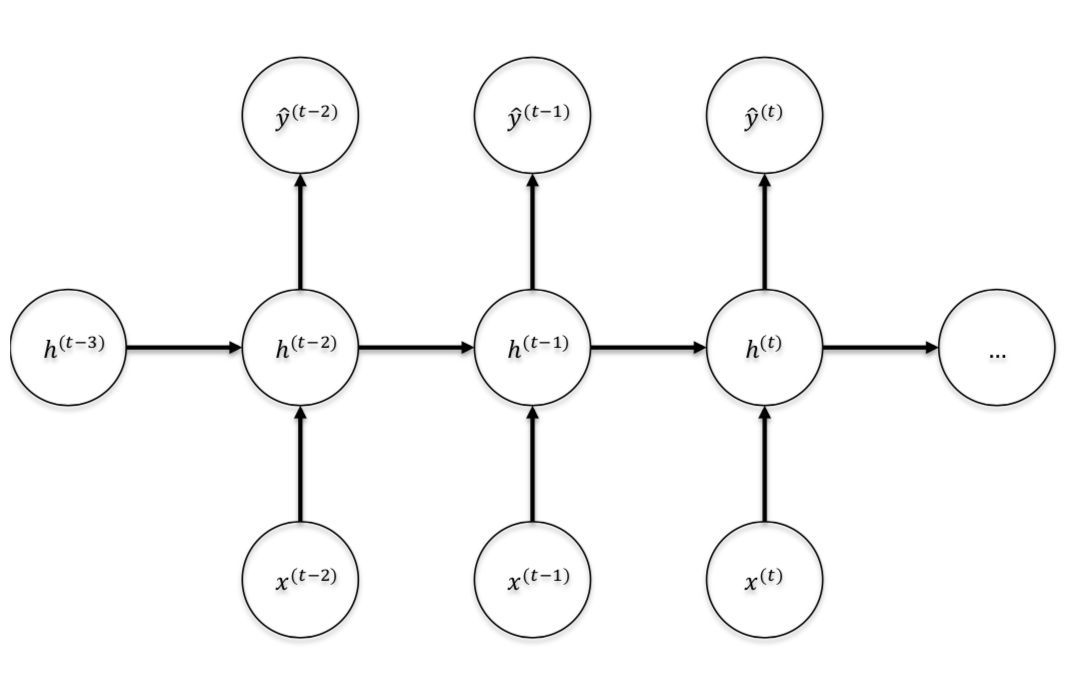
\includegraphics[scale=0.75]{unrolled3timesteps}
\end{figure}
\vskip5em
%----------------------
\subproblem{d}{How Many Operations for Single Timestep (3 points, written)}
\noindent \textbf{Answer:} \\

\noindent Derivatives for the skip-gram model
\begin{align}
	%
	\frac{J_{skip-gram}(word_{c-m \dots c+m})}{\partial \bm{v}_{c}} &= %
		\sum\limits_{-m \leq j \leq m, j \ne 0} \frac{\partial F(\bm{w}_{c+j}, \bm{v}_{c})}{\partial \bm{v}_{c}} \nonumber \\
	%
	\frac{J_{skip-gram}(word_{c-m \dots c+m})}{\partial \bm{v}_{j}} &= 0, \forall j\ne c \nonumber \\
	%
	\frac{J_{skip-gram}(word_{c-m \dots c+m})}{\partial \bm{U}} &= %
		\sum\limits_{-m \leq j \leq m, j \ne 0} \frac{\partial F(\bm{w}_{c+j}, \bm{v}_{c})}{\partial \bm{U}} \nonumber 
\end{align}


\noindent Derivatives for the CBOW model
\begin{align}
	%
	\frac{J_{CBOW}(word_{c-m \dots c+m})}{\partial \bm{v}_{j}} &= %
		\frac{\partial F(\bm{w}_{c}, \hat{\bm{v}})}{\partial \hat{\bm{v}}}, \forall (j \ne c) \in \{c-m \dots c+m\}  \nonumber \\
	%
	\frac{J_{CBOW}(word_{c-m \dots c+m})}{\partial \bm{v}_{j}} &= 0, %
		\forall (j \ne c) \notin \{c-m \dots c+m\}  \nonumber \\
	%
	\frac{J_{CBOW}(word_{c-m \dots c+m})}{\partial \bm{U}} &= %
		\frac{\partial F(\bm{w}_{c}, \hat{\bm{v}})}{\partial \bm{U}} \nonumber
\end{align}

\vskip5em


\newpage
%----------------------
\subproblem{e}{How Many Operations for Entire Sequence (3 points, written)}

\noindent \textbf{Answer:}  See code: $\sim$\verb|/q3_word2vec.py|.

%----------------------
\subproblem{f}{Which largest? Term RNN? (1 point, written)}

\noindent \textbf{Answer:}  See code: $\sim$\verb|/q3_sgd.py|.

%----------------------
\subproblem{g}{Bonus (1 point, written)}
\noindent \textbf{Answer:} \\

\textit {Explain: In the Word Vectors image, words clustered at similarity, such as the emotion words "amazing", "wonderful" and "great" are very close to each other. The word "well" a little further but still close to "amazing"  , the connection characters and words "the" "a" "," etc are spread around alone.
}

\end{document}
